\section{Extraction cost and development quality}
\subsection{Reference design and metrics}
The separate LOC material comes from Chronicling America \citep{loc}. The LOC comparison uses 16 pages with 52 reference claims, including three pages with no forecasts, plus a distinct set of 44 boundary decisions. The reference was produced by a language model following a written protocol before the tested extractor outputs were available. It is model-adjudicated, not human gold. The boundary set contains 32 exclusion traps and 12 awkward but eligible forecasts. Its accuracy is a separate diagnostic, not an alternative estimate of population precision.\evidence{X1}

For matched extracted spans, precision is $TP/(TP+FP)$, recall is $TP/(TP+FN)$, and $F_1=2TP/(2TP+FP+FN)$. The saved evaluator uses greedy one-to-one containment matching at 0.7. The protocol text instead mentions a Jaccard threshold of 0.6; this documentation inconsistency must be resolved before treating the benchmark as a finalized validation package. We report the metrics produced by the saved evaluation, with that limitation disclosed.\evidence{X1}

Whole-page reference annotation makes false negatives observable within those pages. In contrast, reviewing only extracted positive candidates cannot reveal forecasts the extractor never proposed. This difference explains why the LOC experiment reports recall while the ProQuest human review does not. It does not make the model-produced LOC reference more authoritative than human review; the two designs answer different questions.

\begin{table}[t]
\caption{Recorded LOC development cost--quality comparison}\label{tab:cost}
\centering\small
\begin{tabularx}{\linewidth}{Xrrrrr}
\toprule
Configuration & Precision & Recall & F1 & \$/1,000 & \$/23,000\\
\midrule
Regex baseline & .609 & .269 & .373 & 0.00 & 0.00\\
OSS extraction & .536 & .712 & .612 & 0.98 & 22.65\\
OSS + self-verification & .618 & .654 & .636 & 1.17 & 26.82\\
OSS + Lite verification & .756 & .596 & .667 & 1.89 & 43.52\\
OSS + Flash verification & .931 & .519 & .667 & 4.58 & 105.43\\
Flash, one window & 1.000 & .654 & .791 & 12.62 & 290.36\\
Flash, 8k windows & .844 & .731 & .784 & 17.55 & 403.70\\
\bottomrule
\end{tabularx}
\note{USD per number of LOC \emph{pages}, using the historical report's token-based projections. OSS denotes the archived gpt-oss-120b configuration; Lite and Flash denote the archived Gemini Flash-Lite and Flash configurations. Exact run names are in Appendix~\ref{app:cost}. The reference is 16 pages/52 claims, produced by a model; these are development metrics. Zero regex cost means zero metered language-model API charges. It excludes labor and computing. Costs are not current quotations, invoices, or ProQuest article costs. Source: X1.}
\end{table}

\subsection{The observed tradeoff}
The self-verifying OSS pipeline identifies 34 of 52 reference claims and returns 21 unmatched claims: precision 0.618, recall 0.654, and F1 0.636. Its recorded projection is \$26.82 for 23,000 pages. The Flash 8k-window configuration identifies 38 reference claims with seven unmatched claims, yielding precision 0.844, recall 0.731, and F1 0.784 at \$403.70. The cost ratio is about 15.1, or 93.4\% lower projected API cost for the economical configuration. Four more matched claims and fourteen fewer unmatched claims distinguish these particular outputs; the sample is too small and specialized to establish a general ranking.\evidence{X1}

Cost and F1 are not monotonically related. The one-window Flash configuration has F1 0.791 at a lower projected cost than its 8k-window counterpart, though it has lower recall. On the boundary exercise, the 8k configuration resolves 43 of 44 cases, versus 41 for the one-window configuration and 36 for OSS self-verification. Reporting the one-window result is essential: the \$403.70 configuration is a higher-recall comparison, not the unique F1 leader or an unqualified optimum.

\begin{figure}[t]
\centering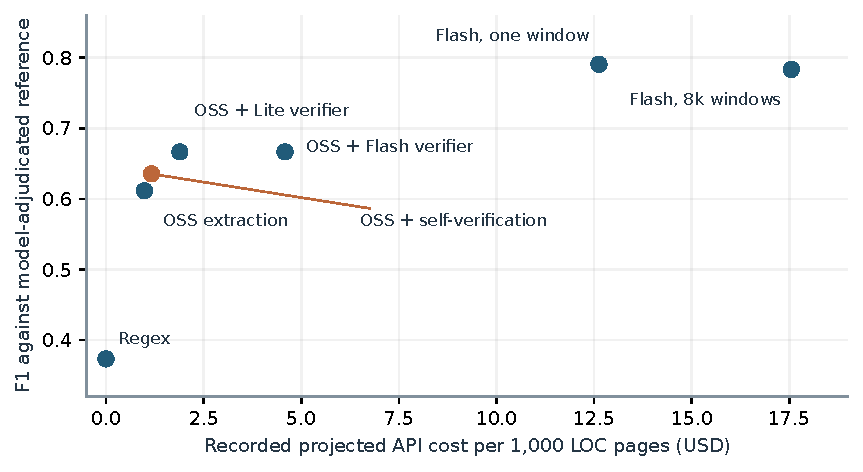
\includegraphics[width=.98\linewidth]{cost_quality.pdf}
\caption{API expenditure and extraction agreement in the LOC development sample. The horizontal axis converts the recorded 23,000-page projections into cost per 1,000 pages. No point represents a ProQuest cost or human-validated F1. The diagram displays observed configurations rather than an estimated population efficiency frontier.}\label{fig:cost}
\end{figure}

Verification changes the composition of errors. Unverified OSS extraction produces 37 true matches and 32 unmatched candidates. Flash verification retains 27 true matches and two unmatched candidates. Precision rises substantially, but ten previously matched claims are lost. A filter cannot recover an omitted candidate unless it also performs a new extraction step. The relevant question is therefore whether reduced false positives justify lost recall for the intended downstream analysis, not whether adding verification is inherently beneficial.

\subsection{Cost accounting and limits to transportability}
For pipeline stages $s$, the recorded projection has the form
\begin{equation}
 C(N)=\frac{N}{16}\sum_s\frac{T_{s,\mathrm{in}}r_{s,\mathrm{in}}+T_{s,\mathrm{out}}r_{s,\mathrm{out}}}{10^6},
 \label{eq:cost}
\end{equation}
where token totals $T$ are measured over the development pages and rates $r$ are the report's historical dollars per million tokens. The formula assumes that token use scales linearly with page count. Different document lengths, retry rates, forecast densities, or output budgets can violate that approximation.

The recorded OSS extraction component is \$22.65 per 23,000 pages. Subtracting it from the rounded pipeline totals gives approximately \$4.17 for self-verification, \$20.87 for Lite verification, and \$82.78 for Flash verification. These are differences of rounded projections, not separately audited bills. The development narrative reports approximately \$0.86 spent on the benchmark, but the cost script sums pipeline costs that reuse extraction stages. Without a reconciled call-level ledger, we cannot certify that figure as unique billed expenditure.\evidence{X1}

Full project cost additionally includes source access, retrieval, failed calls, infrastructure, human review, and interpretation. Local inference removes a provider's per-token charge but does not make hardware, power, or operator time free. No complete ProQuest usage ledger or human-hours record is available in the inspected evidence. Thus, the results support the narrower claim that some extraction configurations have low projected API cost; they do not establish the total cost per valid ProQuest forecast or the savings relative to manual corpus construction.

The reference pages come from a crisis-focused LOC cache. Forecast density, OCR difficulty, publication style, and the mix of advertisements and retrospectives may differ in ordinary periods and in ProQuest articles. The experiment does not establish that those differences leave precision or recall unchanged. A common, human-annotated document sample spanning eras and forecast densities would be needed to test transportability and compare cost per correctly recovered forecast.

